\begin{figure}[!t]
\centering
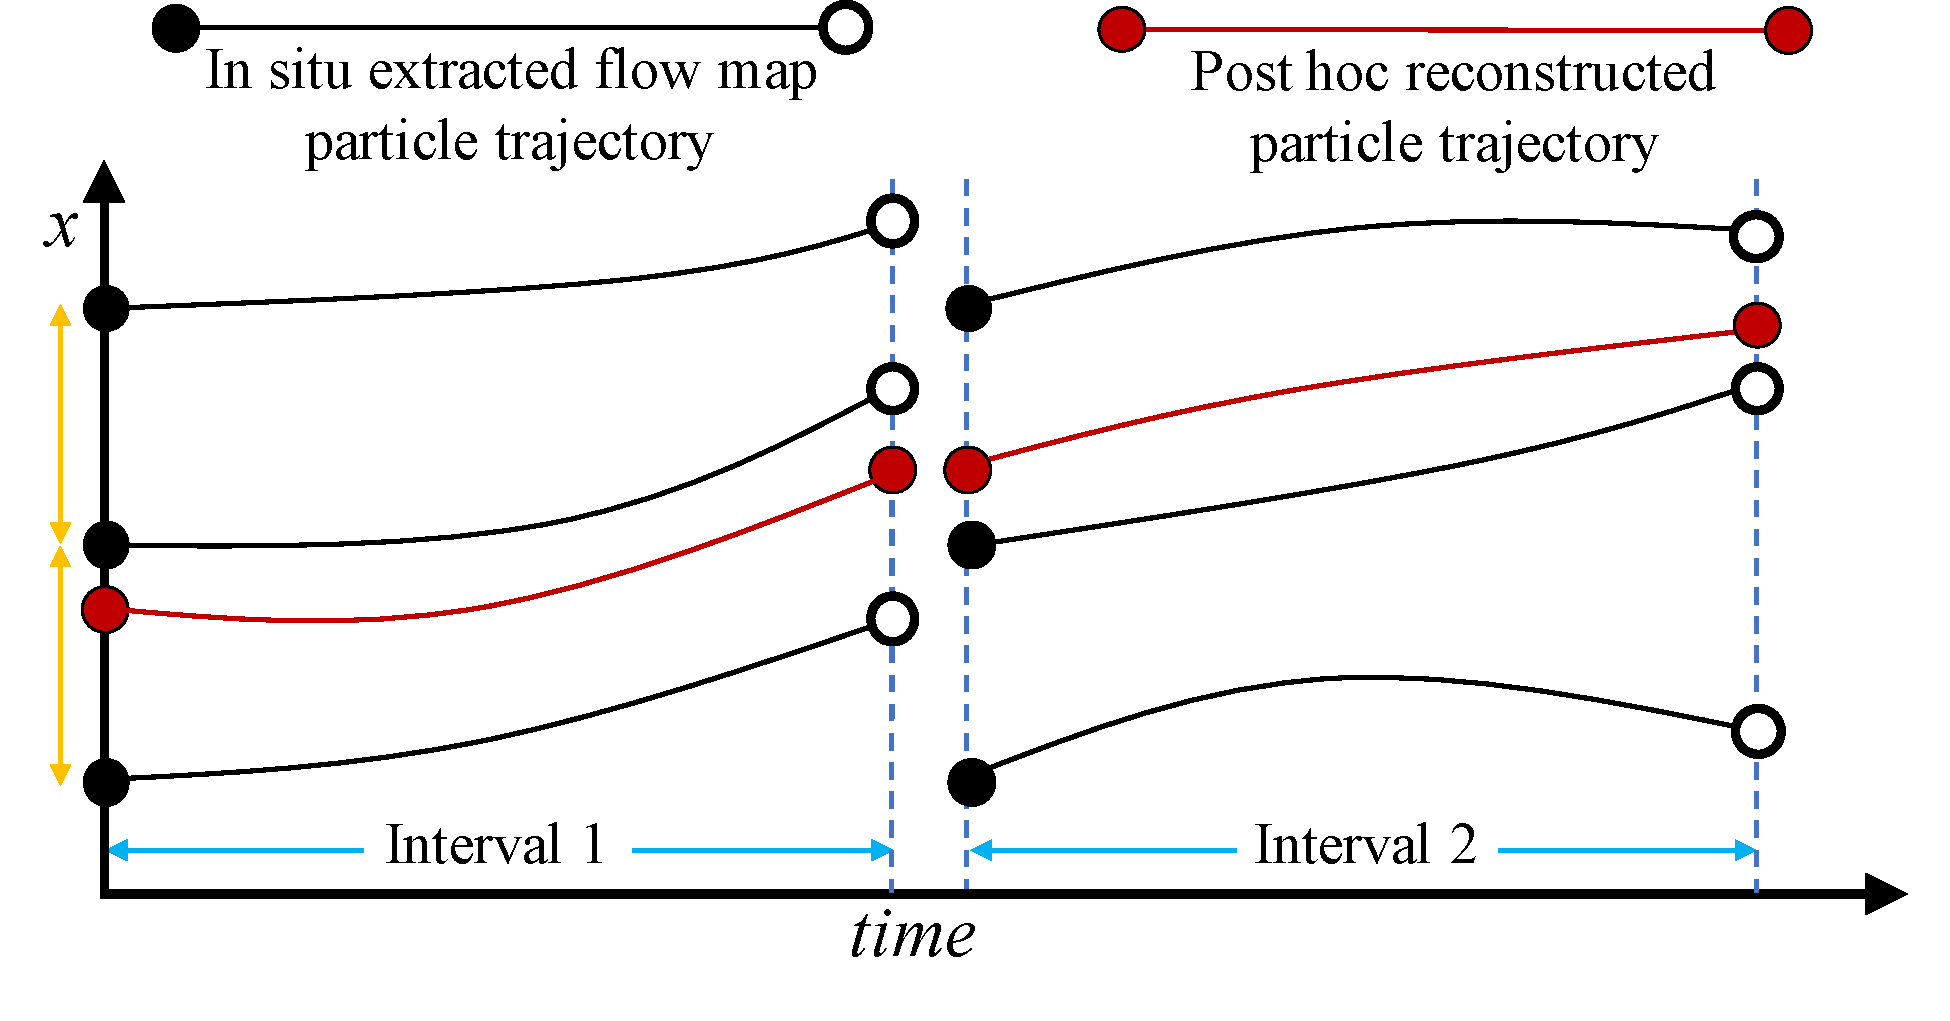
\includegraphics[width=0.95\linewidth]{Images/phases_new.pdf}
\caption{\fix{The phases of Lagrangian analysis. The in situ phase involves using uniform seed placement and extracting flow maps over temporally non-overlapping intervals. The extracted flow maps are used as input for exploratory post hoc phase. In this example, the trajectory of a particle (red) is calculated by interpolating the flow maps over two intervals of time.}}
\vspace{-6mm}
\label{fig:phases}
\end{figure}
